\PassOptionsToPackage{usenames}{xcolor}
\PassOptionsToPackage{dvipsnames}{xcolor}
\documentclass[11pt,a4paper,twoside,final,titlepage,openright]{book}%
\usepackage{beamerarticle}

\usepackage[utf8]{inputenc}
\usepackage[T1]{fontenc}
\usepackage[spanish]{babel}

\usepackage{listings}
\usepackage{palatino}
\usepackage{lmodern}

%\renewcommand*\rmdefault{lmr}
%\renewcommand*\ttdefault{ppl}

\usepackage{url}
\usepackage{multicol}

\usepackage{tikz}
\usetikzlibrary{positioning}
\usetikzlibrary{arrows}
\usetikzlibrary{mindmap}

\usepackage{pgfplots}
\pgfplotsset{compat=1.5}

\usepackage{ccicons}

\tikzset{
  invisible/.style={opacity=0},
  visible on/.style={alt=#1{}{invisible}},
  alt/.code args={<#1>#2#3}{%
    \alt<#1>{\pgfkeysalso{#2}}{\pgfkeysalso{#3}} % \pgfkeysalso doesn't change the path
  },
}



\usepackage[a4paper,left=2cm,right=2cm,top=2.5cm,bottom=4cm]{geometry}
\usepackage[colorlinks=true,linkcolor=blue,citecolor=blue,urlcolor=blue,plainpages=false,bookmarksnumbered=true,pdfpagemode=UseOutlines]{hyperref}


\usepackage[nottoc]{tocbibind}

%\usepackage[fixlanguage]{babelbib}


\usepackage{graphicx}
\usepackage{xcolor}
\usepackage{tikz}
\usetikzlibrary{arrows,positioning} 

\newcommand{\textgood}[1]{%
{\color{blue!60!black}\textbf{#1}}%
}

\newcommand{\textbad}[1]{%
{\color{red!80!black}\textbf{#1}}%
}

\newcommand{\textmark}[1]{%
{\color{orange!70!black}\textbf{#1}}%
}

\newcommand{\textenum}[1]{%
{\color{blue!60!black}\textbf{#1}}%
}

\newcommand{\textemph}[1]{%
{\color{green!40!black}\textbf{#1}}%
}

\newcommand{\versionid}{2020.1}
\newcommand{\versiondate}{Septiembre de 2020}

\newcommand{\coursetitle}{Programación de Altas Prestaciones}
\newcommand{\moduleintro}{Presentación}
\newcommand{\modulefundcap}{Fundamentos de la Computación de Altas Prestaciones}
\newcommand{\modulecopymove}{Tipos Definidos por el Usuario: Copia y Movimiento}
\newcommand{\modulememmgmt}{Gestión avanzada de memoria: Punteros elegantes}
\newcommand{\modulegeneric}{Programación genérica: Polimorfismo estático}


\newtheorem{ejer}{Ejercicio}

\usepackage{url}

\usepackage{pdfpages}

\usepackage{todonotes}

%Package fancyhdr
\usepackage{fancyhdr}
\setlength{\headheight}{1.7cm}%{13.6pt}
\pagestyle{fancyplain}
\fancyhf{}
\lhead{
\includegraphics[height=1.25cm]{logos/uc3m.png}}
\chead{}
\rhead{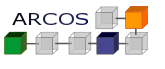
\includegraphics[height=1.25cm]{logos/arcos.png}}
\rfoot{\begin{tabular}{r}\coursetitle\\Versión \versionid\end{tabular}}
\cfoot{\begin{tabular}{c}{\thepage}\\{}\end{tabular}}
\lfoot{
\begin{tabular}{l}
\textbf{\ccbysa} -- CC BY-SA 4.0\\J. Daniel Garcia -- ARCOS@UC3M
\end{tabular}
}
\renewcommand{\headrulewidth}{0.5pt} % remove lines as well
\renewcommand{\footrulewidth}{0.5pt}
\renewcommand{\plainheadrulewidth}{0.5pt}
\renewcommand{\plainfootrulewidth}{0.5pt}

\renewcommand{\topfraction}{0.9}
\renewcommand{\textfraction}{0.1}
\renewcommand{\floatpagefraction}{0.9}

\usepackage{palatino}
\usepackage{lmodern}

\renewcommand*\rmdefault{lmr}
\renewcommand*\ttdefault{ppl}

\makeindex

\begin{document}

\mode<article>{
\lstset{
  language=C++,
  belowcaptionskip=1\baselineskip,
  breaklines=true,
  xleftmargin=\parindent,
  showstringspaces=false,
  basicstyle=\small,
  keywordstyle=\bfseries\color{green!40!black},
  commentstyle=\itshape\color{purple!40!black},
  identifierstyle=\color{blue},
  stringstyle=\color{brown},
  columns=fullflexible,
  inputencoding=utf8,
  extendedchars=true,
  morekeywords=[1]{_Pragma,constexpr,nullptr,alignof,alignas,decltype,override,final,noexcept,deprecated,thread_local,co_await,co_return,co_yiedl},
  literate=%
    {¿}{{?`}}{1}
    {¡}{{!`}}{1}
    {á}{{\'a}}{1}
    {é}{{\'e}}{1}
    {í}{{\'i}}{1}
    {ó}{{\'o}}{1}
    {ú}{{\'u}}{1}
    {ñ}{{\~n}}{1}
}
}

\mode<presentation>{
\lstset{
  language=C++,
  belowcaptionskip=1\baselineskip,
  breaklines=true,
  xleftmargin=\parindent,
  showstringspaces=false,
  basicstyle=\scriptsize,
  keywordstyle=\bfseries\color{green!40!black},
  commentstyle=\itshape\color{purple!40!black},
  identifierstyle=\color{blue},
  stringstyle=\color{orange},
  directivestyle=\bfseries\color{green!40!black},
  columns=fullflexible,
  inputencoding=utf8,
  extendedchars=true,
  morekeywords=[1]{_Pragma,constexpr,nullptr,alignof,alignas,decltype,override,final,noexcept,deprecated,thread_local,co_await,co_return,co_yield},
  literate=%
    {¿}{{?`}}{1}
    {¡}{{!`}}{1}
    {á}{{\'a}}{1}
    {é}{{\'e}}{1}
    {í}{{\'i}}{1}
    {ó}{{\'o}}{1}
    {ú}{{\'u}}{1}
    {ñ}{{\~n}}{1}
}
}

\newcommand{\cppkey}[1]{%
{\color{green!40!black}\textbf{#1}}%
}

\newcommand{\cppid}[1]{%
{\color{blue}\textbf{#1}}%
}

\newcommand{\cppstr}[1]{%
{\color{orange}\textbf{#1}}%
}


\lstdefinestyle{terminal}{
  language=bash,
  basicstyle=\scriptsize\ttfamily,
  numbersep=3pt,
  frame=tb,
  columns=fullflexible,
  backgroundcolor=\color{yellow!20},
}



\frontmatter

\pagestyle{empty}
\begin{titlepage}
\tikz[remember picture,overlay] \draw [fill,Blue] (current page.north west) rectangle +(0.2\paperwidth,-\paperheight);
\begin{flushright}

\includegraphics[width=5cm]{logos/uc3m.png}
\\
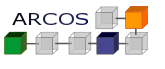
\includegraphics[width=5cm]{logos/arcos.png}
\end{flushright}

\vfill

\begin{tabular}{p{3cm}l}
&
\LARGE{Material de curso}
\\

&\\

&
\LARGE{\coursetitle}
\\

&\\

&
Version: \versionid
\\

&
\versiondate
\\

\end{tabular}
\vfill
\begin{tabular}{p{3cm}l}
&José Daniel García Sánchez\\
&Departamento de Informática\\
&Grupo ARCOS\\
&Universidad Carlos III de Madrid\\
&Av. Universidad, 30\\
&28911 Leganés, Madrid\\
&\url{josedaniel.garcia@uc3m.es}\\
\end{tabular}
\vspace{1cm}
\\
\begin{tabular}{p{3cm}l}
&
%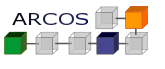
\includegraphics[width=5cm]{logos/arcos.png}
%
\includegraphics[width=8cm]{logos/logo-uc3m.jpg}
\\
\end{tabular}
\end{titlepage}

\pagestyle{fancyplain}
\chapter*{Atribución-CompartirIgual 4.0 Internacional (CC BY-SA 4.0)}

Este es un resumen legible por humanos (y no un sustituto) de la
licencia (código legal disponible en
\url{https://creativecommons.org/licenses/by-sa/4.0/legalcode}
).

\section*{Usted es libre de:}

\begin{itemize}

\item \textbf{Compartir} --
copiar y redistribuir el material en cualquier medio o formato.

\item \textbf{Adaptar} -- 
remezclar, transformar y construir a partir del material
para cualquier propósito, incluso comercialmente.

\end{itemize}

La licenciante no puede revocar estas libertades en tanto usted siga los
términos de la licencia.

\section*{Bajo los siguientes términos:}

\begin{itemize}

\item \ccAttribution \quad \textbf{Atribución} --
Usted debe dar crédito de manera adecuada, brindar un enlace a la licencia, e
indicar si se han realizado cambios. Puede hacerlo en cualquier forma
razonable, pero no de forma tal que sugiera que usted o su uso tienen el apoyo
de la licenciante. 

\item \ccShareAlike \quad \textbf{CompartirIgual} --
Si remezcla, transforma o crea a partir del material, debe distribuir su
contribución bajo la lamisma licencia del original. 

\item \textbf{No hay restricciones adicionales} -- 
No puede aplicar términos legales ni medidas tecnológicas que restrinjan
legalmente a otras a hacer cualquier uso permitido por la licencia. 

\end{itemize}

\section*{Avisos:}

No tiene que cumplir con la licencia para elementos del materiale en el dominio
público o cuando su uso esté permitido por una excepción o limitación
aplicable.

No se dan garantías. La licencia podría no darle todos los permisos que
necesita para el uso que tenga previsto. Por ejemplo, otros derechos como
publicidad, privacidad, o derechos morales pueden limitar la forma en que
utilice el material.


\cleardoublepage
\chapter*{Presentación}

Bienvenidos.

\section*{Estructura}

Pendiente.

\cleardoublepage
\chapter*{Agradecimientos}

En primer lugar, me gustaría dar las gracias a Bjarne Stroustrup
por darnos el lenguaje de programación C++.

También me gustaría expresar mi gratitud a todos los miembreos del
grupo de trabajo ISO/IEC JTC1/SC22/WG21, que han trabajado durante
décadas para mejorar y actualizar el lenguaje.
La discusión con muchos de ellos sobre diversos aspectos específicos
del lenguaje y de la biblioteca estándar han sido para mi de gran utilidad.

Así mismo, me gustaría agradecer de forma especial a todos aquellos
que han proporcionado realimentación sobre versiones previas de este 
material.

Un agradecimiento especial lo merecen todos los estudiantes que han cursad
la asignatura de Programación de Altas Prestaciones.



\cleardoublepage
\tableofcontents
\listoftodos

\mainmatter

\pagestyle{fancyplain}
\mode<article>{\chapter{\moduleintro}}

\section{Profesorado}

\begin{frame}{Coordinador}
\begin{columns}

\column{.4\textwidth}

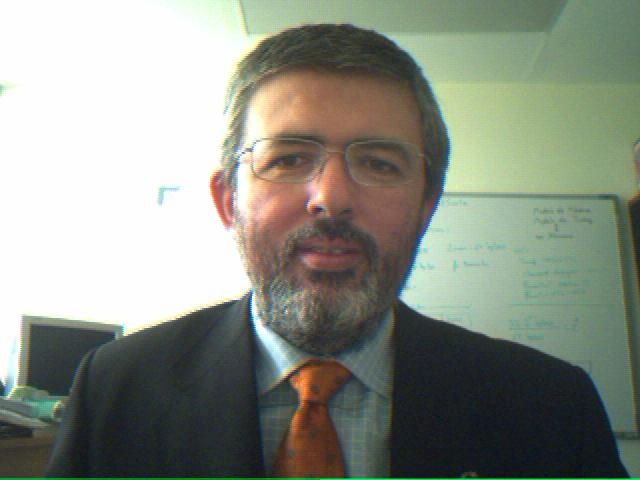
\includegraphics[width=0.8\textwidth]{images/prof/jdgarcia.jpg}

\column{.6\textwidth}

\begin{itemize}
\item José Daniel García Sánchez.
\item Departamento de Informática.
\item Págia Web: \url{https://www.arcos.inf.uc3m.es/wp/jdgarcia}
\end{itemize}

\end{columns}
\end{frame}

\section{Visión general}

\subsection{Objetivos y competencias}

\begin{frame}[t]{Asignatura}
\begin{itemize}
  \item \textmark{Objetivo}: 
  que el estudiante sea capa de usar \textmark{lenguajes y técnicas de programación} que
  permitan obtener \textgood{altas prestaciones} en el contexto del desarrollo de 
  \textgood{software financiero}.

\end{itemize}
\end{frame}

\begin{frame}[t]{Resultados de aprendizaje}
\begin{itemize}
  \item Para alcanzar este objetivo, el estudiante profundizará en aspectos:
    \begin{itemize}
      \vspace{1.5em}
      \pause
      \item Conocer los principales lenguajes de programación que se utilizan para el desarrollo de software financiero.

      \vspace{1.5em}
      \pause
      \item Capacidad para implementar software para el sector financiero.

      \vspace{1.5em}
      \pause
      \item Conocimientos sobre la programación de altas prestaciones.
    \end{itemize}
\end{itemize}
\end{frame}


\subsection{Audiencia}

\begin{frame}{Audicencia}
\begin{itemize}
  \item Programación de Altas Prestaciones.
    \begin{itemize}
      \item Titulación: Master en Tecnologías de la Computación aplicadas al sector financiero.
      \item Tipo: Obligatoria.
      \item Curso: 1.
      \item Cuatrimestre: 1.
      \item Créditos: 6 ECTS.
    \end{itemize}

  \vfill
  \item Conocimientos previos:
    \begin{itemize}
      \item Programación.
      \item Arquitectura de Computadores.
      \item Estructuras de Datos.
      \item Sistemas Operativos.
    \end{itemize}
\end{itemize}
\end{frame}

\subsection{Programa de contenidos}

\begin{frame}[t]{Programa}
\begin{enumerate}
  \item Fundamentos de la Computación de Altas Prestaciones.
  \item Lenguajes de Programación.
  \item Gestión de Memoria.
  \item Programación genérica.
  \item Bibliotecas e interoperabilidad.
  \item Optimización de código.
  \item Análisis del rendimiento.
  \item Hilos y frameworks de concurrencia y paralelismo.
\end{enumerate}
\end{frame}

\section{Recursos}

\begin{frame}[t]{Bibliografía}
\begin{itemize}
  \item Bibliografía básica:
    \begin{itemize}
      \item Bjarne Stroustrup. Programming – Principles and Practice. 2nd Edition. Addison-Wesley. 2014.
      \item Anthony Williams. C++ Concurrency in Action. Practical Multithreading. Manning. 2nd Edition. 2019.
      \item Michael Voss, Rafael Asenjo, James Reinders. Pro TBB: C++ Parallel Programming with Threading Building Blocks. APress. 2019.
    \end{itemize}
  \vspace{1em}
  \pause
  \item \footnotesize Bibliografía adicional:
    \begin{itemize}
      \item \tiny Bjarne Stroustrup. The C++ Programming Language. 4th Edition. Addison-Wesley. 2013.
      \item \tiny Bjarne Stroustrup. A Tour of C++. Addison-Wesley. 2nd Edition. 2018.
      \item \tiny Michael Voss et al. 
      \item \tiny Gerassimos Barlas. Multicore and GPU Programming: An Integrated Approach. Morgan-Kaufmann. 2014
      \item \tiny Peter Gottschling. Discovering Modern C++: An intensive course for scientists, engineers and programmers. Addison-Wesley. 2015
      \item \tiny Kurt Guntheroth. Optimized C++. O’Reilly. 2016
      \item \tiny Carlos Oliveira. Practical C++ Financial Programming. Apress. 2015.
    \end{itemize}
\end{itemize}
\end{frame}


\section{Evaluación}

\begin{frame}[t]{Sistema de evaluación}
\begin{itemize}
  \item Resumen:
  \vspace{1em}
    \begin{itemize}
      \item Examen final: 30\% de la calificación final.
        \begin{itemize}
          \item Incluye todos los contenidos (teoría, prácticas, y proyectos).
        \end{itemize}

      \item Evaluación continua: 70\% de la calificación final.
        \begin{itemize}
          \item Tests de evaluación: 30\% de la calificación final.
          \item Prácticas en grupo: 40\% de la calificación final.
        \end{itemize}
    \end{itemize}
  \vspace{1em}
  \begin{itemize}
    \item Convocatorias:
      \begin{itemize}
        \item Convocatoria ordinaria: Enero.
        \item Convocatoria extraordinaria: Junio.
      \end{itemize}
  \end{itemize}
\end{itemize}
\end{frame}

\begin{frame}[t]{Evaluación continua}
\begin{itemize}
  \item Obtener buen resultado en la evaluación continua es clave para superar la asignatura.
  \item Elementos:
    \begin{itemize}
      \item Tests de evaluación: 30\% de la calificación final.
      \item Prácticas: 40\% de la calificación final.
    \end{itemize}
  \vspace{1em}
  \item No has seguido la evaluación continua si:
    \begin{itemize}
      \item Obtienes menos de 3.5 en la media de todas las prácticas.
    \end{itemize}
\end{itemize}
\end{frame}

\begin{frame}[t]{Convocatoria ordinaria: Evaluación continua}
\begin{itemize}
  \item Si sigues el proceso de evaluación continua:
    \begin{itemize}
    \item Examen final: 30\%.
      \begin{itemize}
        \item Mínimo necesario: 3.0.
      \end{itemize}
    \item Tests de evaluación: 30\%
      \begin{itemize}
        \item Mínimo necesario: \alert{No hay mínimo}.
      \end{itemize}
    \item Prácticas: 40\%.
      \begin{itemize}
        \item Mínimo en la media de todas las prácticas: 3.5.
      \end{itemize}
    \item Si no logras algún mínimo, la media no se calcula y serás calificado como suspenso.
  \end{itemize}
  \item \alert{Bonus}:
    \begin{itemize}
      \item Se añadirá 1.5 puntos adicionales a la calificación final si:
        \begin{itemize}
          \item Obtienes al menos 7.0 puntos en la evaluación continua, y además
          \item obtienes al menos 6.0 puntos en el examen final.
        \end{itemize}
    \end{itemize}
\end{itemize}
\end{frame}

\begin{frame}[t]{Convocatoria ordinaria: Evaluación NO-continua}
\begin{itemize}
  \item Si no has seguido el proceso de evaluación continua:
    \begin{itemize}
      \item El examen final tiene un valor del 60\% de la calificación final.
      \item Necesitarás 8.33 en ele examen final para superar la asignatura.
    \end{itemize}
  \item \alert{CONSEJO}:
    \begin{itemize}
      \item Pon esfuerzo en seguir el proceso de evaluación continua.
    \end{itemize}
\end{itemize}
\end{frame}


\begin{frame}[t]{Convocatoria extraordinaria}
\begin{itemize}
  \item Examen extraordinario en el mes de junio.
  \vspace{1em}
  \item Normas:
    \begin{enumerate}
      \item Estudiantes que han completado el proceso de evaluación continua:
        \begin{itemize}
          \item El examen final vale el 30\% y la evaluación continua el otro 70\%.
          \item Solamente se aplica si la calificación en el examen es de al menos 3.5.
        \end{itemize}
      \item Estudiantes que no han completado el proceso de evaluación continua:
        \begin{itemize}
          \item El examen vale el 100\%.
        \end{itemize}
    \end{enumerate}
    \begin{itemize}
      \item A los estudiantes que hayan completado el proceso de evaluación continua se tomará la opción más favorable.
    \end{itemize}
\end{itemize}
\end{frame}

\begin{frame}[t]{Pruebas de evaluación}
\begin{itemize}
  \item \alert{MUY IMPORTANTE}:
    \begin{itemize}
      \item La no asistencia al examen final implica la calificación como NO-PRESENTADO, independientemente de cualquier otra calificación.
    \end{itemize}
\end{itemize}
\end{frame}


\mode<article>{\chapter{\modulefundcap}}

\section{Introducción}

\begin{frame}[t]{La ley de Moore}
\begin{columns}
  \begin{column}{.5\textwidth}
    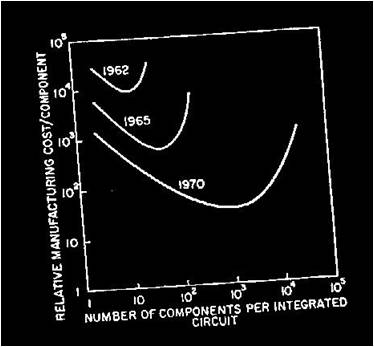
\includegraphics[width=.5\textwidth]{images/moore-graph1.jpg}\\
    \begin{flushright}
      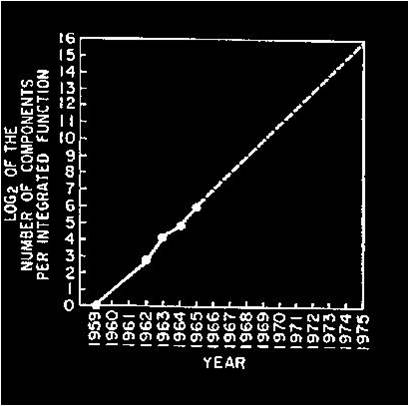
\includegraphics[width=.65\textwidth]{images/moore-graph2.jpg}\\
    \end{flushright}
  \end{column}
  \begin{column}{.5\textwidth}
    \begin{itemize}
    \item El número de transistores por chip se duplica cada N meses.
      \begin{itemize}
        \item Donde 12 \textless N \textless 24.
        \item Gordon Moore, 1965.
      \end{itemize}
    \end{itemize}
    \vspace{1em}
    \begin{center}
      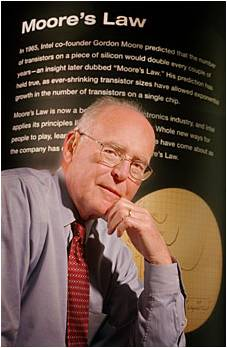
\includegraphics[width=.4\textwidth]{images/gordon-moore.jpg}
    \end{center}
  \end{column}
\end{columns}
\end{frame}



\begin{frame}[t]{Transistores por chip}
    \begin{center}
      \mode<presentation>{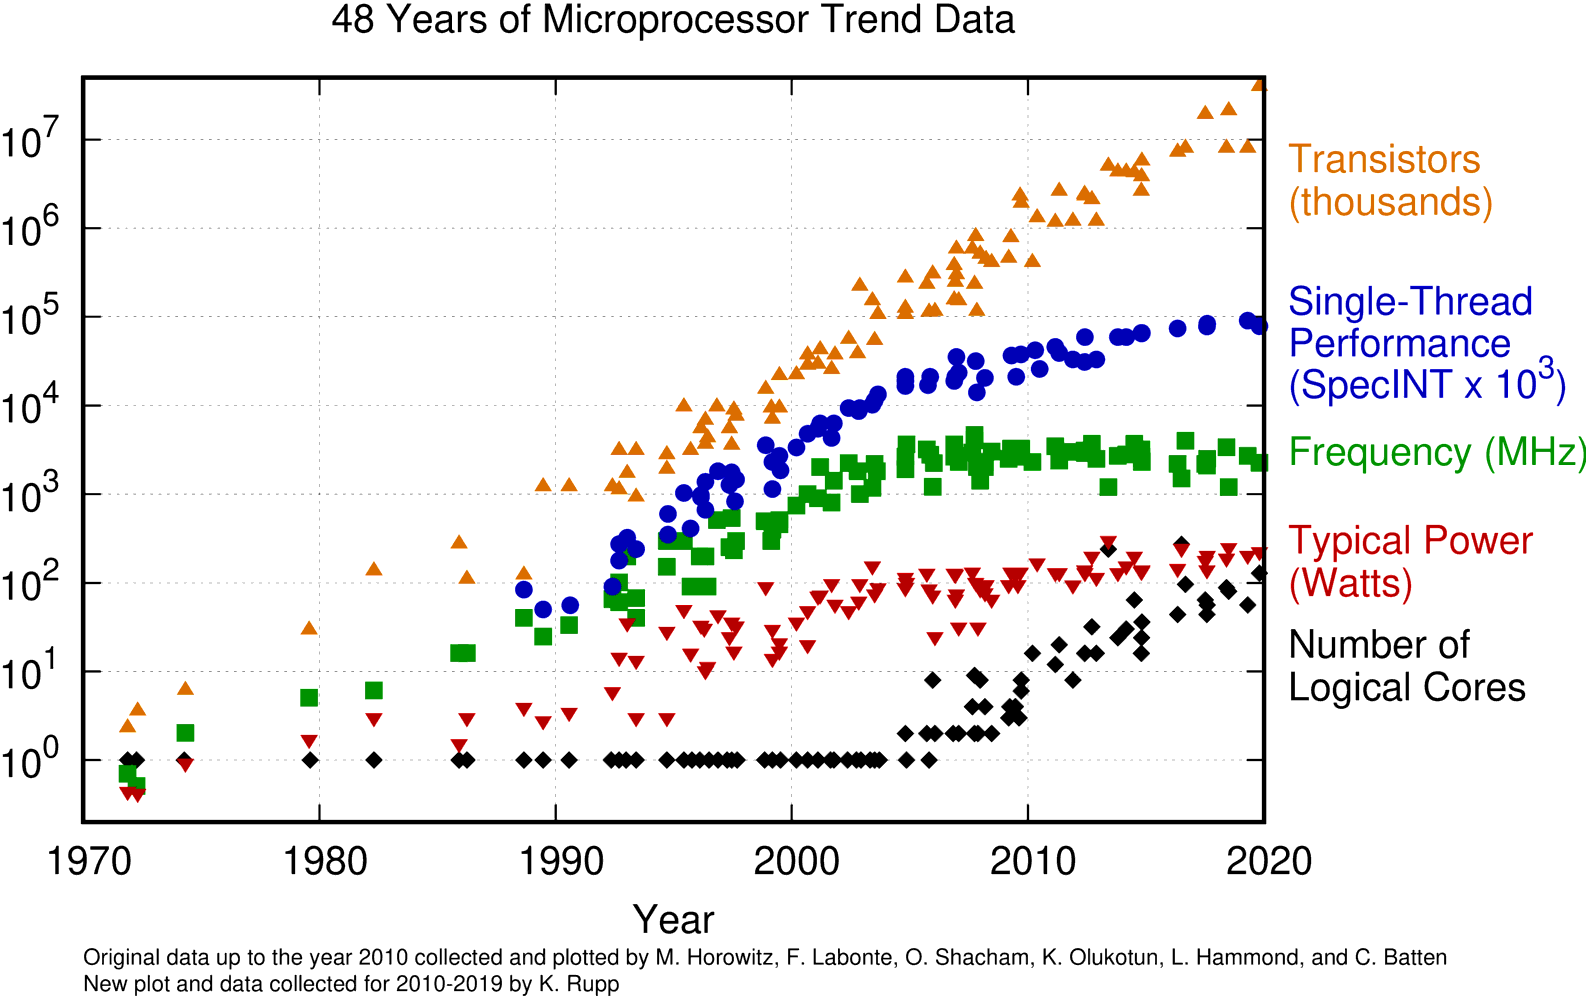
\includegraphics[height=.8\textheight]{images/48-years-processor-trend.png}}
      \mode<article>{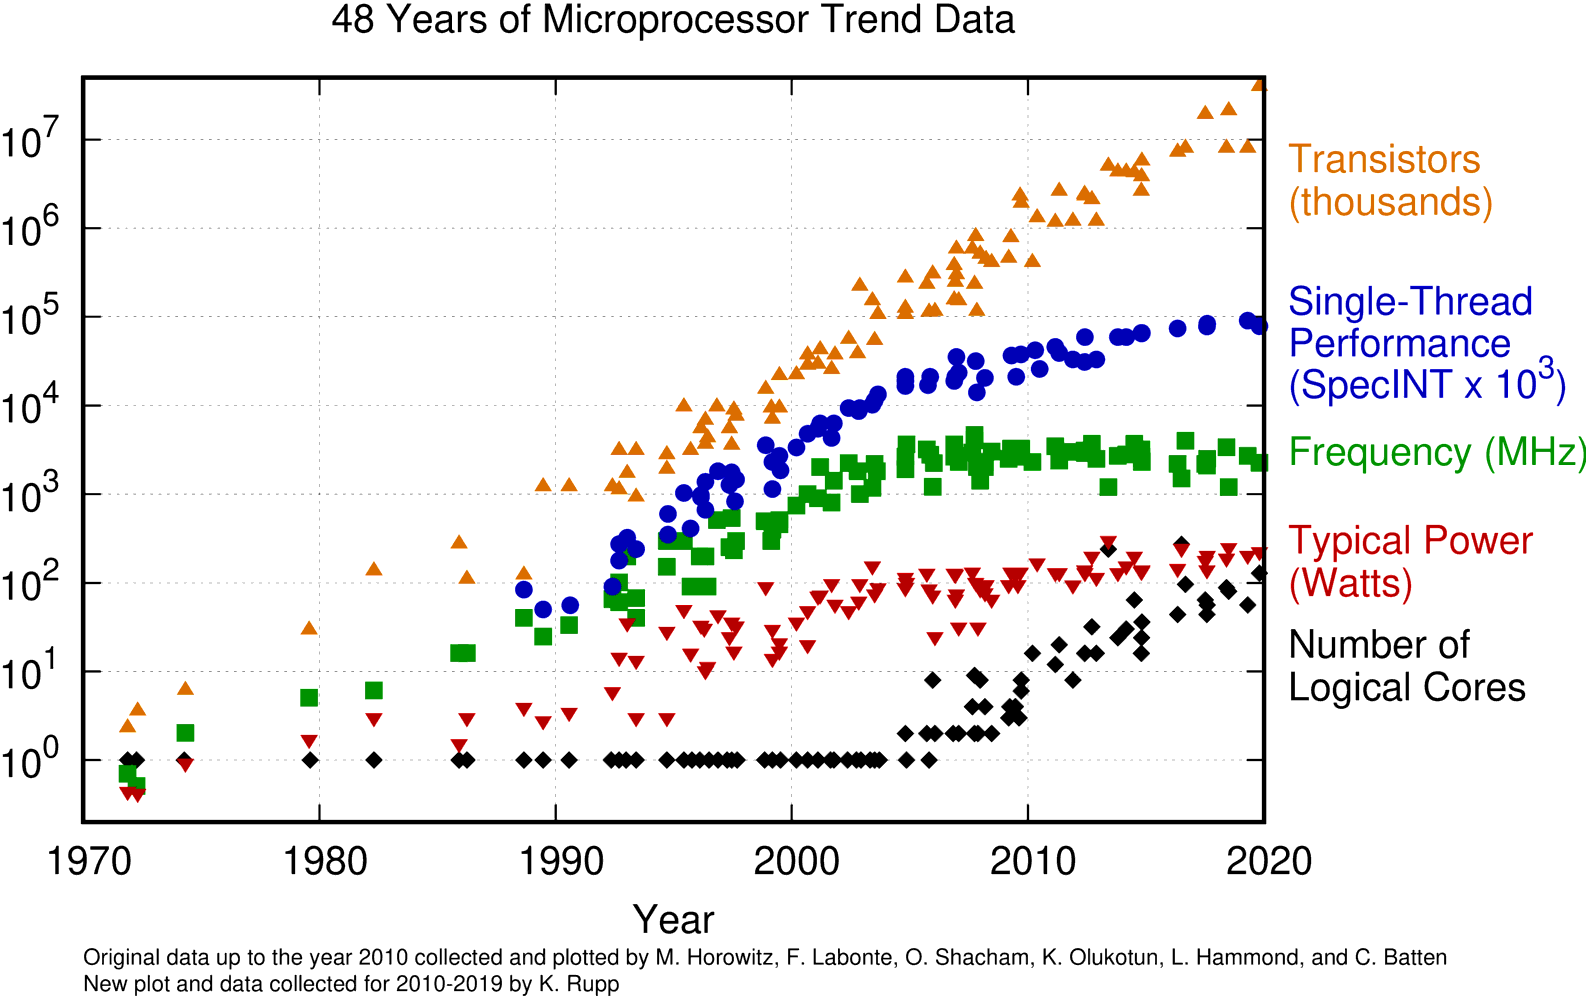
\includegraphics[height=.8\textwidth]{images/48-years-processor-trend.png}}
    \end{center}
\end{frame}

\begin{frame}[t]{The free lunch is over}
    \begin{itemize}
      \item Actividad: Lea completamente el artículo:
    \end{itemize}
    \vspace{2em}
    Fuente: \alert{The free lunch is over}.\\
    Herb Sutter.\\
    \url{http://www.gotw.ca/publications/concurrency-ddj.htm}\\
\end{frame}

\begin{frame}{Evolución del rendimiento}
\begin{columns}
  \begin{column}{.75\textwidth}
    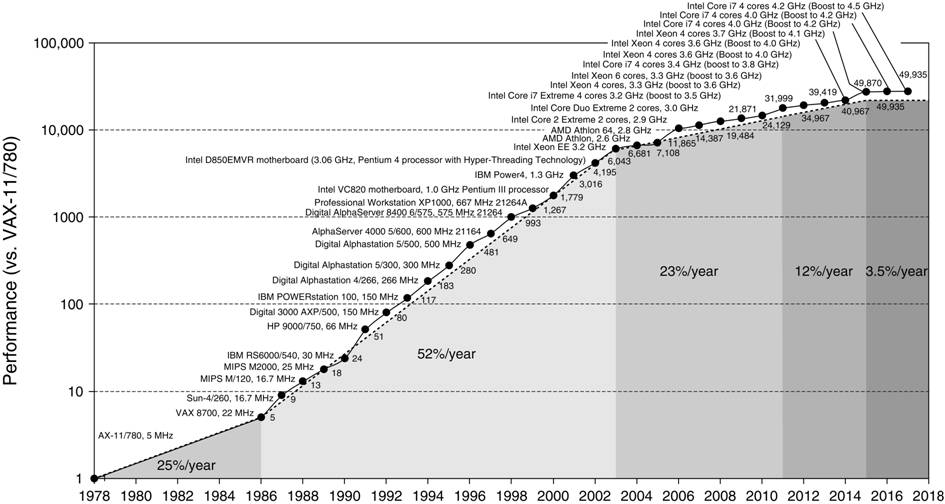
\includegraphics[width=\textwidth]{images/perf-evol.jpg}\\
    {\tiny Fuente: Computer Architecture: A Quantitative Approach. 5 Ed
Hennessy and Patterson. Morgan Kaufmann. 2012.}
  \end{column}
  \begin{column}[T]{.25\textwidth}
    \begin{itemize}
      \item 1986: \alert{RISC}.
      \item 2005: \alert{multi-core}.
    \end{itemize}
  \end{column}
\end{columns}
\end{frame}

\begin{frame}[t]{La revolución RISC}
\begin{itemize}
  \item Mejora continua de semiconductores ha dado lugar al dominio de computadores 
        basados en microprocesador.
    \mode<presentation>{\vfill}
    \begin{itemize}
      \item Desaparición de los minicomputadores.
      \mode<presentation>{\vfill}
      \item \emph{Mainframes} y supercomputadores construidos como colecciones de microprocesadores.
    \end{itemize}
  \mode<presentation>{\pause\vfill}
  \item Incremento sostenido del rendimiento de 1986 a 2003:
    \begin{itemize}
      \item \textbf{\alert{52\% anual}}.
    \end{itemize}
  \mode<presentation>{\pause\vfill}
  \item \textbf{¡Ha dejado de cumplirse!}
\end{itemize}
\end{frame}

\section{Evaluación del rendimiento}

\input{02-fundcap/perf-metrics}
\input{02-fundcap/benchmarks}
\input{02-fundcap/amdahl}
\input{02-fundcap/gustaffson}

\section{Altas prestaciones en aplicaciones secuenciales}

\begin{frame}[t]{Efectos de las arquitecturas segmentadas}
\begin{itemize}
  \item La mayoría de los procesadores hoy día usan arquitecturas segmentadas (\emph{pipeline}).
  \item Esto provoca detenciones para evitar:
    \begin{itemize}
      \item Riesgos de datos: Los accesos a datos provocan detenciones
        \begin{itemize}
          \item Especialmente si no se encuentran en la caché.
        \end{itemize}
      \item Riesgos de control: Las bifurcaciones condicionales provocan detenciones.
        \begin{itemize}
          \item Mitigado en parte con el predictor de saltos.
          \item Uso por el compilador de desenrrollamiento de bucles.
        \end{itemize}
    \end{itemize}
\end{itemize}
\end{frame}

\begin{frame}[t]{Memoria caché}
\begin{itemize}
  \item Memorias de acceso rápido (normalmente en el propio chip).
  \item Aprovechamiento del principio de localidad:
    \begin{itemize}
      \item Localidad espacial.
      \item Localidad temporal.
    \end{itemize}
  \item Objetivo: Obtener una alta tasa de aciertos en caché.
\end{itemize}
\end{frame}

\begin{frame}[t]{¿Cómo aprovechar la caché?}
\begin{itemize}
  \item El compilador ya usa técnicas de aprovechamiento de la caché:
    \begin{itemize}
      \item Código: reordenación de rutinas, alinear bloques básicos a líneas de caché, linearización de saltos, \ldots
      \item Datos: Fusión de bucles, intercambio de bucles, \ldots
    \end{itemize}
  \vfill
  \item Pero el desarrollador puede ayudar:
    \begin{itemize}
      \item Organización de arrays multidimensionales.
      \item Acceso a matrices por bloques.
      \item Evitar uso excesivo de memoria dinámica.
    \end{itemize}
\end{itemize}
\end{frame}

\section{Paralelismo y altas prestaciones}

\begin{frame}[t]{¿Por qué TLP?}
\begin{itemize}
  \item Algunas aplicaciones presentan más \textgood{paralelismo natural} que 
        el que se puede conseguir con \textmark{arquitecturas segmentadas}.
    \begin{itemize}
      \item Servidores, aplicaciones científicas, \ldots
    \end{itemize}

  \mode<presentation>{\vfill\pause}
  \item Emergen \textenum{dos modelos}:
    \begin{itemize}
      \item \textgood{Paralelismo a nivel de hilos (TLP)}:
        \begin{itemize}
          \item \textmark{Hilo}: Proceso con sus propias instrucciones y datos.
          \item Puede ser parte un programa o programa independiente.
          \item Cada hilo tiene asociado su \textmark{estado} 
                (instrucciones, datos, PC, registros, \ldots).
        \end{itemize}
      \item \textgood{Paralelismo a nivel de datos (DLP)}:
        \begin{itemize}
          \item Operaciones idénticas sobre distintos datos.
        \end{itemize}
    \end{itemize}
\end{itemize}
\end{frame}

\begin{frame}[t]{TLP}
\begin{itemize}
  \item \textgood{ILP} explota paralelismo implícito dentro un bloque básico
        o en bucles.

  \mode<presentation>{\vfill}
  \item \textgood{TLP} utiliza múltiples hilos de ejecución que son 
        inherentemente paralelos.

  \mode<presentation>{\vfill\pause}
  \item \textenum{Objetivo de TLP}:
    \begin{itemize}
      \item Utilizar múltiples flujos de instrucciones para mejorar:
        \begin{itemize}
          \item \textmark{Tasa de procesamiento} de computadores que ejecutan muchos programas.
          \item \textmark{Tiempo de ejecución} de programas multi-hilo.
        \end{itemize}
    \end{itemize}
\end{itemize}
\end{frame}

\begin{frame}[t]{Ejecución multi-hilo}
\begin{itemize}
  \item Múltiples hilos comparten las unidades funcionales de un procesador solapando su uso.
    \begin{itemize}
      \item Necesidad de replicar n-veces el estado.
        \begin{itemize}
          \item Banco de registros, PC, tabla de páginas (si hilos no pertenecen al mismo programa).
          \item Memoria compartida mediante mecanismos de memoria virtual.
          \item Hardware para cambio de hilo rápido.
        \end{itemize}

      \mode<presentation>{\vfill\pause}
      \item \textenum{Tipos}:
        \begin{itemize}
          \item \textmark{Grano fino}: Cambio de hilo en cada instrucción.
          \item \textmark{Grano grueso}: Cambio de hilo en detenciones (ej. Fallo de caché).
          \item \textmark{Multi-hilo simultáneo}: Grano fino con emisión múltiple y planificación dinámica.
        \end{itemize}
    \end{itemize}
\end{itemize}
\end{frame}

\begin{frame}[t]{Multi-hilo de grano fino}
\begin{itemize}
  \item Se alterna entre hilos en cada instrucción.
    \begin{itemize}
      \item Se entrelaza la ejecución de los hilos.
      \item Normalmente se hace \emph{round-robin}.
      \item Se excluyen de \emph{round-robin} hilos en detención (\emph{stall}).
      \item El procesador debe poder cambiar de hilo en cada ciclo de reloj.
    \end{itemize}

  \mode<presentation>{\vfill\pause}
  \item \textgood{Ventaja}:
    \begin{itemize}
      \item Puede ocultar detenciones cortas y largas.
    \end{itemize}

  \mode<presentation>{\vfill}
  \item \textbad{Desventaja}:
    \begin{itemize}
      \item Retrasa la ejecución de hilos individuales por reparto.
    \end{itemize}

  \mode<presentation>{\vfill}
  \item \textmark{Ejemplo}: Sun Niagara.
\end{itemize}
\end{frame}

\begin{frame}[t]{Multi-hilo de grano grueso}
\begin{itemize}
  \item Cambia de hilo solamente en detenciones largas.
    \begin{itemize}
      \item \textmark{Ejemplo}: Fallo en caché L2.
    \end{itemize}

  \mode<presentation>{\vfill\pause}
  \item \textgood{Ventajas}:
    \begin{itemize}
      \item No hace falta cambio de hilo excesivamente rápido.
      \item No retrasa hilos individuales.
    \end{itemize}

  \mode<presentation>{\vfill}
  \item \textbad{Desventajas}:
    \begin{itemize}
      \item Se debe vaciar o congelar el pipeline.
      \item Se debe llenar el pipeline con instrucciones del nuevo hilo (latencia).
    \end{itemize}

  \mode<presentation>{\vfill}
  \item Apropiado cuando rellenado del pipeline tarda mucho menos que tiempo de detención.
    \begin{itemize}
      \item \textmark{Ejemplo}: IBM AS/400.
    \end{itemize}
\end{itemize}
\end{frame}

\begin{frame}[t]{SMT: Multi-hilo simultáneo}
\begin{itemize}
  \item \textgood{Idea}: Procesadores con planificación dinámica 
        ya tienen muchos mecanismo de soporte para multi-hilo.
    \begin{itemize}
      \item Grandes conjuntos de registros virtuales.
        \begin{itemize}
          \item Registros para múltiples hilos.
        \end{itemize}
      \item Renombrado de registros.
        \begin{itemize}
          \item Evita mezcla en acceso a registros de hilos.
        \end{itemize}
      \item Finalización fuera de orden.
    \end{itemize}

  \mode<presentation>{\vfill\pause}
  \item \textenum{Modificaciones}:
    \begin{itemize}
      \item Tabla de renombrado por hilo.
      \item Registros PC separados.
      \item ROB separados.
    \end{itemize}

  \mode<presentation>{\vfill}
  \item \textmark{Ejemplos}: Intel Core i7, IBM Power 7

\end{itemize}
\end{frame}

\begin{frame}[t]{TLP: Resumen}
\makebox[\textwidth][c]{
\input{02-fundcap/tlp-alt.tkz}
}
\end{frame}


\mode<article>{\chapter{\modulecopymove}}

\section{Desarrollo de un vector de números}

\begin{frame}[t]{Objetivo}
\begin{itemize}
\item En esta unidad iremos incorporando los conceptos al desarrollo de un tipo \cppid{vector}.
\item La idea es desarrollar un tipo con funcionalidad parecida a \cppid{vector<double>}.
\end{itemize}
\end{frame}

\mode<presentation>{

\begin{frame}
\begin{block}{vector.h}
\lstinputlisting[lastline=18]{03-copymove/vec1/vector.h}
\end{block}
\end{frame}

\begin{frame}
\begin{block}{vector.h}
\lstinputlisting[firstline=20]{03-copymove/vec1/vector.h}
\end{block}
\end{frame}

}

\mode<article>{

\begin{frame}
\begin{block}{vector.h}
\lstinputlisting{03-copymove/vec1/vector.h}
\end{block}
\end{frame}

}

\mode<presentation>{

\begin{frame}
\begin{block}{vector.cpp}
\lstinputlisting[lastline=14]{03-copymove/vec1/vector.cpp}
\end{block}
\end{frame}

\begin{frame}
\begin{block}{vector.cpp}
\lstinputlisting[firstline=16]{03-copymove/vec1/vector.cpp}
\end{block}
\end{frame}

}

\mode<article>{
\begin{frame}
\begin{block}{vector.cpp}
\lstinputlisting[lastline=15]{03-copymove/vec1/vector.cpp}
\end{block}
\end{frame}
}

\begin{frame}
\begin{block}{main.cpp}
\lstinputlisting{03-copymove/vec1/main.cpp}
\end{block}
\mode<presentation>{
\begin{itemize}
\item \pause \alert{¿Problemas?}
\end{itemize}
}
\end{frame}

\begin{frame}[fragile]{Comprobación de memoria}
\begin{itemize}
  \item \alert{valgrind}: Conjunto de herramientas para realizar análisis dinámico de programas.
  \item \alert{memcheck}: Herramienta para:
    \begin{itemize}
      \item Accesos indebidos a memoria.
      \item Usos peligrosos de valore no iniciados.
      \item Goteos de memoria.
      \item Errores en liberación de memoria.
    \end{itemize}
  \item Invocación:
\begin{lstlisting}[style=terminal]
valgrind --tool=memcheck programa
\end{lstlisting}
\begin{lstlisting}[style=terminal]
...
==15344== HEAP SUMMARY:
==15344==     in use at exit: 40 bytes in 1 blocks
==15344==   total heap usage: 1 allocs, 0 frees, 40 bytes allocated
==15344== LEAK SUMMARY:
==15344==    definitely lost: 40 bytes in 1 blocks
...
\end{lstlisting}
\end{itemize}
\end{frame}

\section{Destructores}

\begin{frame}[fragile]{El problema de la desasignación}
\begin{itemize}
  \item Un tipo que adquiere recursos (ej. memoria) y no lo libera provoca un goteo de memoria.
  \item Solución simple:
    \begin{itemize}
      \item Función miembro de liberación.
    \end{itemize}
\begin{lstlisting}
class vector {
  // ...
  void libera() { delete []v; }
  // ...
};

int main() {
  vector v{5};
  // ...
  v.libera();
}
\end{lstlisting}
\end{itemize}
\end{frame}

\begin{frame}[fragile]{Función miembro de destrucción}
\begin{itemize}
  \item Un \alert{destructor} es una función miembro especial que se ejecuta 
        \textbf{de forma automática} cuando un objeto sale de alcance.
    \begin{itemize}
      \item No tiene tipo de retorno.
      \item No toma parámetros.
      \item Su nombre es el nombre de clase precedido del símbolo \cppkey{\~}.
    \end{itemize}
\begin{lstlisting}
class vector {
  // ...
  ~vector() { delete []v; }
  // ...
};
\end{lstlisting}
  \item Invocación automática.
\begin{lstlisting}
void f() {
  vector v{10};
  rellena(v);
  cout << v << endl;
} // Invoca al destructor de v
\end{lstlisting}
\end{itemize}
\end{frame}

\begin{frame}[fragile]{Destrucción generado por defecto}
\begin{itemize}
  \item En realidad todos los tipos tienen una función miembro destructor.
    \begin{itemize}
      \item El compilador genera una que es válida en la mayoría de los casos.
    \end{itemize}
  \item Dado un tipo sin destructor, el compilador \emph{sintetiza} uno:
    \begin{itemize}
      \item Invoca (recursivamente) al destructor de cada miembro.
      \item El destructor de un tipo primitivo es la operación nula.
    \end{itemize}
\end{itemize}
\begin{lstlisting}
struct estudiante {
  string nombre;
  vector<double> notas;
  // ...
};

void f() {
  estudiante e { "Carlos", {9.0, 9.5, 8.5} };
  cout << e.nombre << " -> " << e.notas[0] << endl;
} // Destrucción de e
\end{lstlisting}
\end{frame}

\section{Constructores}

\subsection{Tipos sin constructor}

\begin{frame}[fragile]{Iniciación sin constructor}
\begin{itemize}
  \item Iniciación de tipos primitivos.
\begin{lstlisting}
int x{1024}; // int x = 1024
double * p{nullptr}; // double * p = nullptr
\end{lstlisting}
  \item Clases que no tienen constructor:
\begin{lstlisting}
struct dispositivo {
  string id_serie;
  long long capacidad;
};
\end{lstlisting}
    \begin{itemize}
      \item Iniciación por miembros:
\begin{lstlisting}
dispositivo d1{"hda1", 1024};
\end{lstlisting}
      \item Iniciación por copia
\begin{lstlisting}
dispositivo d3{d1}; // Copia miembro a miembro
\end{lstlisting}
      \item Iniciación por defecto
\begin{lstlisting}
dispositivo d4{};
dispositivo d5;
\end{lstlisting}
    \end{itemize}
\end{itemize}
\end{frame}

\begin{frame}[fragile]
\begin{itemize}
  \item Si se usa iniciación por defecto:
    \begin{itemize}
      \item Variables globales $\rightarrow$ iniciación por defecto de miembros
\begin{lstlisting}
dispositivo d1; // id_serie="", capacidad=0
dispositivo d2{}; // id_serie="", capaciad=0
\end{lstlisting}
      \item Variables locales $\rightarrow$ iniciación por defecto de miembros de tipo clase
        \begin{itemize}
          \item Miembros de tipos primitivos sin iniciar.
        \end{itemize}
\begin{lstlisting}
void f() {
  dispositivo d3; // id_serie="", capacidad=?
  dispositivo d4{}; // id_sere="", capacidad=0
}
\end{lstlisting}
    \end{itemize}
  \item Se puede indicar valor por defecto para miembros.
\begin{lstlisting}
struct dispositivo {
  string id_serie{"sda1"};
  long long capacidad{1024};
};
\end{lstlisting}
\end{itemize}
\end{frame}

\subsection{Tipos con constructor}

\begin{frame}[fragile]{Invocación al constructor}
\begin{itemize}
  \item Sin un tipo tiene uno o más constructores, todas las definiciones de objetos 
        deben invocar algún constructor.
    \begin{itemize}
      \item El compilador deja de generar un constructor por defecto.
    \end{itemize}
\begin{lstlisting}
struct complejo {
  double real, imag;
  complejo(double r);
  complejo(double r, double i);
};

complejo c1; // Error
complejo c2{}; // Error
complejo c3{2.0}; // OK
complejo c4{2.0, 3.5}; // OK
complejo * pc = new complejo{2.0,3.5}; // OK
complejo v[] { {1.0,1.5}, {2.0, 2.0} }; // OK
vector<complejo> w { {1.0, 1.5}, {2.0, 2.0} }; // OK
\end{lstlisting}
\end{itemize}
\end{frame}

\begin{frame}[fragile]
\begin{itemize}
  \item Existe una sintaxis para forzar la invocación de un constructor.
    \begin{itemize}
      \item No invoca iniciación miembro a miembro o basadas en lista.
    \end{itemize}
\begin{lstlisting}
struct punto {
  double x, y;
};
punto p1(1.0, 1.0); // Error: No hay constructor
punto p2{1.0, 1.0}; // OK
punto p3(1.0); // Error: No hay constructor
punto p4{1.0}; // x=1.0, y=0.0
complejo c1(1.0, 1.0); // OK
complejo c2{1.0, 1.0}; // OK
complejo c3(1.0); // OK
complejo c4{1.0}; // OK
\end{lstlisting}
  \item Útil para discriminar entre constructores de \cppid{std::vector} de tipos numéricos.
\begin{lstlisting}
vector<int> v{10}; // Vector con el valor 10. v.size() == 1
vector<int> v(10); // Vector con 10 valores 0. v.size() == 10
\end{lstlisting}
\end{itemize}
\end{frame}

\subsection{Constructor por defecto}

\begin{frame}[fragile]
\begin{itemize}
  \item El \alert{constructor vacío} o \alert{constructor por defecto} es un constructor que no toma ningún parámetro.
\begin{lstlisting}
vector();
\end{lstlisting}
  \item Define que debe hacerse:
    \begin{itemize}
      \item Cuando se define un objeto sin valor inicial.
\begin{lstlisting}
vector v;
vector v{};
\end{lstlisting}
      \item Cuando se asigna memoria sin valor inicial
\begin{lstlisting}
vector * pv = new vector;
\end{lstlisting}
      \item El constructor vacío se genera si no hay ningún constructor.
        \begin{itemize}
          \item Se puede inhibir la generación del constructor vacío.
\begin{lstlisting}
vector() = delete;
\end{lstlisting}
          \item Se puede forzar la generación del constructor vacío.
\begin{lstlisting}
vector() = default;
\end{lstlisting}
        \end{itemize}
    \end{itemize}
\end{itemize}
\end{frame}

\begin{frame}[fragile]{Constructor por defecto y arrays}
\begin{itemize}
  \item El tipo base de un array debe tener constructor por defecto, si hace falta iniciar por defecto.
\begin{lstlisting}
struct punto {
  double x, y;
  punto();
};
struct complejo {
  double real, imag;
  complejo(double d, double i);
};

punto v[16]; // OK
complejo w[16]; // Error: No pueden iniciarse elementos
complejo z[] = { {1.0, 1.0}, {2.0, 2.0} }; // OK 
\end{lstlisting}
\end{itemize}
\end{frame}

\begin{frame}[fragile]{Constructor por defecto y vectores}
\begin{itemize}
  \item El tipo base de un vector debe tener constructor por defecto, si hace falta iniciar por defecto.
\begin{lstlisting}
struct punto {
  double x, y;
  punto();
};
struct complejo {
  double real, imag;
  complejo(double d, double i);
};

vector<punto> vp1; // OK. No necesita iniciar
vector<complejo> vc1; // OK. No necesita iniciar

vector<punto> vp2(16); // OK. 16 elementos con valor por defecto
vector<complejo> vc2(16); // Error: no puede iniciar 16 elementos
vector<complejo> vc3{ {1.0, 1.0}, {2.0, 2.0} }; // OK
vector<complejo> vc4{5, {1.0,1.0}}; // OK: 5 elementos iniciados
\end{lstlisting}
\end{itemize}
\end{frame}

\subsection{Conversión y constructor explícito}

\begin{frame}[fragile]{Constructor explícito}
\begin{itemize}
  \item Un constructor que toma un único argumento define una operación de conversión.
\begin{lstlisting}
class complejo {
  complejo(double r, double i);
  complejo(dobule r);
  // ...
};

complejo c = 3.5; // Conversión a complejo
\end{lstlisting}
  \item Sin embargo:
\begin{lstlisting}
vector v = 5; // Conversión de entero a vector
\end{lstlisting}
  \item Se puede forzar a que un constructor no actúe como operación de conversión:
\begin{lstlisting}
explicit vector(int n);
\end{lstlisting}
\end{itemize}
\end{frame}

\subsection{Constructor basado en lista}

\begin{frame}[fragile]{Lista de iniciación}
\begin{itemize}
  \item Un \alert{constructor basado en lista} es un constructor que toma un único argumento de tipo
        \cppid{std::initializer\_list}.
    \begin{itemize}
      \item Permiten definir la construcción de objetos a partir de una lista homogénea de valores.
    \end{itemize}
\begin{lstlisting}
lista l { 1, 2, 3, 4 }; // Invoca a lista(initializer_list<int>)
\end{lstlisting}
  \item Cualquier función puede tomar como parámetro una lista de iniciación.
    \begin{itemize}
      \item El argumento debe pasarse por valor.
    \end{itemize}
\begin{lstlisting}
int maximo(initializer_list<int> l);

void f() {
  x = maximo({1, 3, 4, 2});
  // ...
}
\end{lstlisting}
\end{itemize}
\end{frame}

\begin{frame}[fragile]{\texttt{initializer\_list}}
\begin{itemize}
  \item La clase \cppid{std::initializer\_list} ofrece funciones miembro para acceder a los valores de la lista:
    \begin{itemize}
      \item \cppid{begin()}: Puntero al principio de la lista.
      \item \cppid{end()}: Puntero al final de la lista (siguiente del último).
      \item \cppid{size()}: Tamaño de la lista.
    \end{itemize}
  \item Son suficientes para recorrer la lista:
\begin{lstlisting}
void imprime(std::initializer_list<int> l) {
  for (auto p=l.begin(); p!=l.end(); ++p) {
    cout << * p << endl;
  }
}
\end{lstlisting}
  \item O mejor:
\begin{lstlisting}
void imprime(std::initializer_list<int> l) {
  for (auto x : l) {
    cout << x << endl;
  }
}
\end{lstlisting}
\end{itemize}
\end{frame}

\subsection{Constructores para \texttt{vector}}

\begin{frame}{Constructores}
\begin{itemize}
  \item Constructor vacío
  \item Constructor con tamaño pasa a ser explícito.
  \item Constructor con lista de iniciación.
\end{itemize}
\begin{block}{vector.h}
\mode<presentation>{
\lstinputlisting[firstline=6,lastline=10]{03-copymove/vec2/vector.h}
}
\mode<article>{
\lstinputlisting[firstline=6,lastline=10]{03-copymove/vec2/vector.h}
}
\end{block}
\end{frame}

\begin{frame}
\begin{block}{vector.cpp}
\mode<presentation>{
\lstinputlisting[lastline=16]{03-copymove/vec2/vector.cpp}
}
\mode<article>{
\lstinputlisting{03-copymove/vec2/vector.cpp}
}
\end{block}
\end{frame}

\section{Mecanismos de copia}

\subsection{Copia por defecto}

\begin{frame}[fragile]{Operaciones de copia generadas}
\begin{itemize}
  \item Por cada tipo se generan de forma automática dos operaciones de copia:
    \begin{itemize}
      \item Construcción de copia.
\begin{lstlisting}
T y;
T x{y}; // Construcción de copia
\end{lstlisting}
      \item Asignación de copia.
\begin{lstlisting}
T x, y;
x = y; // Asignación de copia
\end{lstlisting}
    \end{itemize}
  \item Implementación por defecto:
    \begin{itemize}
      \item Invocación (recursiva) de operaciones de copia para cada miembro.
      \item La copia de tipos primitivos es la copia del valor.
    \end{itemize}
  \item ¿Es esto lo adecuado para nuestro \cppid{vector}?
\end{itemize}
\end{frame}

\begin{frame}[fragile]
\begin{block}{main.cpp}
\lstinputlisting{03-copymove/vec3/main.cpp}
\end{block}
\begin{lstlisting}[style=terminal]
0 0 5 0 3.5 
0 0 5 0 3.5 
*** glibc detected *** ./test: double free or corruption (fasttop): 
0x0000000001022010 ***
\end{lstlisting}
\end{frame}

\begin{frame}[fragile]
\begin{lstlisting}[style=terminal]
valgrind ./test
\end{lstlisting}
\begin{lstlisting}[style=terminal,basicstyle=\tiny\ttfamily]
==22680== Memcheck, a memory error detector
==22680== Copyright (C) 2002-2011, and GNU GPL'd, by Julian Seward et al.
==22680== Using Valgrind-3.7.0 and LibVEX; rerun with -h for copyright info
==22680== Command: ./test
==22680== 
0 0 5 0 3.5 
0 0 5 0 3.5 
==22680== Invalid free() / delete / delete[] / realloc()
==22680==    at 0x4C2A09C: operator delete[](void*) (in /usr/lib/valgrind/vgpreload_memcheck-amd64-linux.so)
==22680==    by 0x400C66: vector::~vector() (in /home/jdaniel/Dropbox/cursos/intro-cpp11/init/vec2/test)
==22680==    by 0x400BB5: main (in /home/jdaniel/Dropbox/cursos/intro-cpp11/init/vec2/test)
==22680==  Address 0x5a06040 is 0 bytes inside a block of size 40 free'd
==22680==    at 0x4C2A09C: operator delete[](void*) (in /usr/lib/valgrind/vgpreload_memcheck-amd64-linux.so)
==22680==    by 0x400C66: vector::~vector() (in /home/jdaniel/Dropbox/cursos/intro-cpp11/init/vec2/test)
==22680==    by 0x400BA9: main (in /home/jdaniel/Dropbox/cursos/intro-cpp11/init/vec2/test)
==22680== 
==22680== 
==22680== HEAP SUMMARY:
==22680==     in use at exit: 0 bytes in 0 blocks
==22680==   total heap usage: 1 allocs, 2 frees, 40 bytes allocated
==22680== 
==22680== All heap blocks were freed -- no leaks are possible
==22680== 
==22680== For counts of detected and suppressed errors, rerun with: -v
==22680== ERROR SUMMARY: 1 errors from 1 contexts (suppressed: 2 from 2)
\end{lstlisting}
\end{frame}

\begin{frame}
\begin{itemize}
  \item \alert{Problema}: Al realizar la copia, se ha copiado la dirección del array.
    \begin{itemize}
      \item Los dos vectores están compartiendo el mismo array.
      \item Se está desasignando dos veces un mismo bloque de memoria.
    \end{itemize}
\end{itemize}
\begin{tikzpicture}
\tikzset{
    bloque/.style={rectangle,draw=black, top color=white, bottom color=blue!50,
                   very thick, inner sep=0.5em, minimum size=0.6cm, text centered, font=\tiny},
    flecha/.style={->, >=latex', shorten >=1pt, thick},
    etiqueta/.style={text centered, font=\tiny} 
}  
\node[bloque] (bsize) {5};
\node[bloque,right=0cm of bsize] (bptr) { };
\node[bloque,right=0.5cm of bptr] (v0) {0.0};
\node[bloque,right=0cm of v0] (v1) {0.0};
\node[bloque,right=0cm of v1] (v2) {5.0};
\node[bloque,right=0cm of v2] (v3) {0.0};
\node[bloque,right=0cm of v3] (v4) {3.5};
\draw[flecha] (bptr) -- (v0);
\node[etiqueta, left=0.1cm of bsize] {v1:};
\node[etiqueta, above=0cm of bsize] {tam};

\node[bloque, below=1cm of bsize] (bsize2) {5};
\node[bloque,right=0cm of bsize2] (bptr2) { };
\draw[flecha] (bptr2) -- (v0);
\node[etiqueta, left=0.1cm of bsize2] {v2:};

\end{tikzpicture}
\end{frame}

\subsection{Operaciones de copia}

\begin{frame}[fragile]{Constructor de copia}
\begin{itemize}
  \item El \alert{constructor de copia} se invoca cuando se construye un objeto
        a partir de otro.
    \begin{itemize}
      \item Toma un argumento referencia constante al tipo.
\begin{lstlisting}
vector(const vector &);
\end{lstlisting}
    \end{itemize}
  \item Se puede suprimir la generación automática del constructor de copia.
\begin{lstlisting}
vector(const vector &) = delete;
\end{lstlisting}
  \item El constructor de copia se invocará en definiciones del tipo:
\begin{lstlisting}
vector w {v};
vector w = v;
vector w(v);
\end{lstlisting}
\end{itemize}
\end{frame}

\begin{frame}{Implementación de constructor de copia}
\begin{block}{vector.cpp}
\lstinputlisting[firstline=17,lastline=22]{03-copymove/vec4/vector.cpp}
\end{block}
\end{frame}

\begin{frame}[fragile]{Operador de asignación de copia}
\begin{itemize}
  \item El \alert{operador de asignación de copia} se invoca cuando se asigna un objeto a otro.
    \begin{itemize}
      \item Toma un argumento referencia constante al tipo.
      \item Devuelve una referencia al objeto asignado.
      \item Debe ser una función miembro de la clase.
\begin{lstlisting}
vector & operator=(const vector &);
\end{lstlisting}
    \end{itemize}
  \item Se puede suprimir la generación automática del operador de asignación de copia.
\begin{lstlisting}
vector & operator=(const vector &) = delete;
\end{lstlisting}
  \item El constructor de copia se invocará en definiciones del tipo:
\begin{lstlisting}
w = v;
\end{lstlisting}
\end{itemize}
\end{frame}

\begin{frame}{Implementación de operador de asignación de copia}
\begin{block}{vector.cpp}
\lstinputlisting[firstline=24,lastline=31]{03-copymove/vec4/vector.cpp}
\end{block}
\end{frame}

\begin{frame}{El puntero \emph{this}}
\begin{itemize}
  \item \cppkey{this} es una palabra reservada que se puede evaluar dentro de cualquier función miembro de una clase.
  \item Se evalúa a la dirección de memoria del objeto para el que se está ejecutando la función miembro.
  \item La expresión \cppkey{return *this} en el operador de asignación de copia devuelve una referencia la objeto.
  \item ¿Por qué?
    \begin{itemize}
      \item v1 = v2 = v3;
    \end{itemize}
\end{itemize}
\end{frame}



\section{Operaciones de movimiento}

\subsection{Introducción}

\begin{frame}[fragile]{Intercambio de dos valores}
\begin{itemize}
  \item Función de intercambio para enteros
\begin{lstlisting}
void intercambia(int & x, int & y) {
  int aux{x};
  x = y;
  y = aux;
}

int a = 2, b = 4;
intercambia(a,b); // a=4, b=2
\end{lstlisting}
  \item Se realizan 3 copias de enteros.
\end{itemize}
\end{frame}

\begin{frame}[fragile]
\begin{itemize}
  \item Intercambio de vectores
\begin{lstlisting}
void intercambia(vector & v, vector & w) {
  vector aux{v};
  v = w;
  w = aux;
}
\end{lstlisting}
  \item Operaciones:
    \begin{enumerate}
      \item Construcción por copia de \cppid{aux} $\rightarrow$ 1 asignación de memoria.
      \item Asignación a \cppid{x} $\rightarrow$ 1 desasignación + 1 asignación de memoria.
      \item Asignación a \cppid{y} $\rightarrow$ 1 desasignación + 1 asignación de memoria.
      \item Destrucción de \cppid{tmp} $\rightarrow$ 1 desasignación de memoria
      \item 3 copias del vector elemento a elemento.
    \end{enumerate}
  \item Sin embargo:
    \begin{itemize}
      \item Sería suficiente con intercambiar tamaños y punteros
    \end{itemize}
\end{itemize}
\end{frame}

\begin{frame}[fragile]
\begin{itemize}
  \item Intercambio de vectores (si se tuviese acceso a implementación):
\begin{lstlisting}
void intercambia(vector & v, vector & w) {
  unsigned long aux_tam{v.tam};
  v.tam = w.tam;
  w.tam = aux.tam;
  double * aux_vec = v.vec;
  v.vec = w.vec;
  w.vec = aux.vec;
}
\end{lstlisting}
  \item Operaciones:
    \begin{enumerate}
      \item 0 asignaciones de memoria.
      \item 0 desasignaciones de memoria.
      \item 3 copias de enteros (3 palabras).
      \item 3 copias de puntero (3 palabras).
      \item 0 copias de contenidos de vector.
    \end{enumerate}
  \item Sin embargo:
    \begin{itemize}
      \item Sería necesario acceder a la implementación.
      \item Hay más casos de uso.
    \end{itemize}
\end{itemize}
\end{frame}

\begin{frame}[fragile]{Operaciones de movimiento}
\begin{itemize}
  \item Una operación de movimiento adquiere los recursos de un objeto y lo deja en un estado válido, pero vacío.
    \begin{itemize}
      \item Lo único que se espera de un objeto después es que pueda destruirse.
    \end{itemize}
  \item Operaciones de movimiento:
    \begin{itemize}
      \item Constructor de movimiento: Mueve el objeto origen al objeto creado.
      \item Asignación de movimiento: Mueve el objeto origen al objeto destino.
    \end{itemize}
  \item Orígenes de movimiento:
    \begin{itemize}
      \item Retorno de valores locales por copia.
      \item Variables a las que se aplica \cppid{std::move()}.
    \end{itemize}
\end{itemize}
\end{frame}

\begin{frame}[fragile]{Retorno de objetos locales}
\begin{itemize}
  \item Cuando una función devuelve una copia de un objeto local.
\begin{lstlisting}
string concatena(const string & a, const string & b) {
  string tmp = a + " -- " + b;
  return tmp; // Invoca una operación de movimiento.
}

x = concatena("Daniel", "Garcia");
\end{lstlisting}
  \item Se aprovecha el hecho de que \cppid{tmp} se va a destruir.
    \begin{itemize}
      \item Se transfieren los recursos al destino.
        \begin{itemize}
          \item Ejemplo: Copiando el valor del puntero.
        \end{itemize}
      \item Se deja al origen en un estado \emph{destruible}.
        \begin{itemize}
          \item Ejemplo: Haciendo el puntero \cppkey{nullptr}.
        \end{itemize}
    \end{itemize}
\end{itemize}
\end{frame}

\begin{frame}[fragile]{Aplicación explicita de movimiento}
\begin{itemize}
  \item Cuando se invoca sobre una variable la operación \cppid{std::move()}.
\begin{lstlisting}
void f() {
  string c = "Daniel";
  string d = "Garcia";
  d = std::move(c); // d == "Daniel", c == "Garcia" o vacía
} // Destructores
\end{lstlisting}
  \item Se informa que una variable puede moverse.
    \begin{itemize}
      \item Son las operaciones de movimiento (constructor) y (asignación) las
            que realizan el movimiento.
    \end{itemize}
\end{itemize}
\end{frame}

\subsection{Operaciones de movimiento}

\begin{frame}[fragile]{Constructor de movimiento}
\begin{itemize}
  \item El \alert{constructor de movimiento} se invoca cuando se construye un objeto
        a partir de una operación de movimiento.
    \begin{itemize}
      \item Toma un argumento de tipo \emph{referencia a r-valor}.
    \end{itemize}
\begin{lstlisting}
vector(vector &&);
\end{lstlisting}
  \item Se puede suprimir la generación automática del constructor de movimiento.
\begin{lstlisting}
vector(vector &&) = delete;
\end{lstlisting}
  \item Se puede forzar la generación automática del constructor de movimiento.
\begin{lstlisting}
vector(vector &&) = default;
\end{lstlisting}
  \item Se invoca en contextos como:
\begin{lstlisting}
vector v = f(); // vector f();
vector w = std::move(v);
\end{lstlisting}
\end{itemize}
\end{frame}

\begin{frame}[fragile]{Operador de asignación de movimiento}
\begin{itemize}
  \item El \alert{operador de asignación de movimiento} se invoca cuando se asigna un objeto
        a partir de una operación de movimiento.
    \begin{itemize}
      \item Toma un argumento de tipo \emph{referencia a r-valor}.
    \end{itemize}
\begin{lstlisting}
vector & operator=(vector &&);
\end{lstlisting}
  \item Se puede suprimir la generación automática del operador de asignación de movimiento.
\begin{lstlisting}
vector & operator=(vector &&) = delete;
\end{lstlisting}
  \item Se puede forzar la generación automática del operador de asignación de movimiento.
\begin{lstlisting}
vector & operator=(vector &&) = default;
\end{lstlisting}
  \item Se invoca en contextos como:
\begin{lstlisting}
v = f(); // vector f();
w = std::move(v);
\end{lstlisting}
\end{itemize}
\end{frame}

\begin{frame}{Implementación de constructor de movimiento}
\begin{block}{vector.cpp}
\lstinputlisting[firstline=35,lastline=41]{03-copymove/vec5/vector.cpp}
\end{block}
\end{frame}

\begin{frame}{Implementación de asignación de movimiento}
\begin{block}{vector.cpp}
\lstinputlisting[firstline=43,lastline=47]{03-copymove/vec5/vector.cpp}
\end{block}
\end{frame}




\chapter{Ejercicios}



\nocite{*}
\bibliographystyle{abbrv}
\bibliography{bib/cppref}

\end{document}
